\chapter{Motivation und Ziele}
\label{cha:Motivation_und_Ziele}

In diesem Kapitel wird die Motivation und die gesetzten Ziele der vorliegenden  Arbeit aufgezeigt.

Am \textit{Institute for Energy Efficient Buildings and Indoor Climate }(EBC) wird in Kooperation mit dem \textit{Lehrstuhl für Wärme- und Stoffübertragung }(WSA) verschiedene Abtaumethoden für vereiste Luftkühler erforscht. Der Auftraggeber und Kooperationspartner für die Forschungsarbeiten ist der \textit{Forschungsrat Kältetechnik e.V}. Die komplette Projektumgebung ist in der Abbildung \ref{fig:Projektumgebung} dargestellt

\begin{figure}[htb]
	\centering
		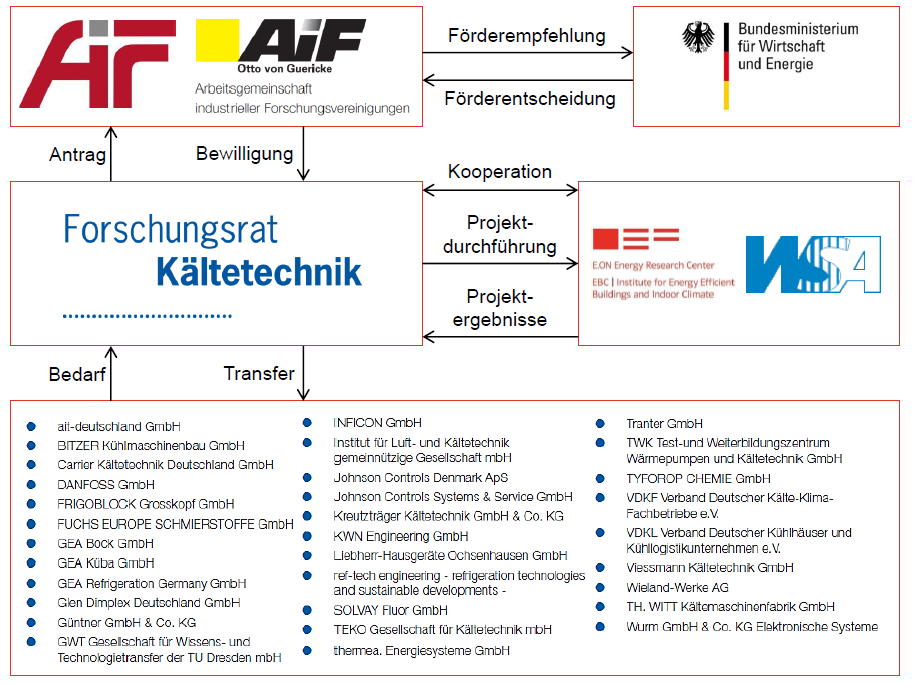
\includegraphics[width=0.80\textwidth]{Pictures/Projektumgebung.png}
	\caption{Projektumgebung für den EBC Abtauprüfstand \citep{Freitag2015}}
	\label{fig:Projektumgebung}
\end{figure}

Die Motivation zu diesem Forschungsprojekt rührt aus dem simplen Phänomen, dass bei der Unterschreitung des Taupunktes der zu kühlenden, vorbeiströmenden Luft zunächst eine Bereifung des Luftkühlers stattfindet. Die Bereifung führt bei einer Verdampfungstemperatur kleiner als 0 °C und somit Unterschreitung des Gefrierpunktes zu einer Vereisung. Die Bereifung führt durch Querschnittsverengungen im Wärmeübertrager des Luftkühlers zu einer erhöhten Strömungsgeschwindigkeit. Diese führt zunächst zu einem erhöhten Wärmeübergang und somit zu einer höhren übertragenden Leistung vom Luftkühler auf die Luft.\citep{Schydlo2010} 

Eine spätere Bereifung der Lamellen führt zu einem sinkenden Wärmeübergang zwischen der Lamelle und der Luft, da sich das gefrorene Eis aufgrund der geringen Wärmeleitfähigkeit wie ein Isolator verhält. Um den eintretenden Leistungsabfall zu kompensieren, wird die Regelung der Kälteanlage die Verdampfungstemperatur verringern. Eine geringere Verdampfungstemperatur bedeutet einen geringeren Betriebssaugdruck, den der Kompressor bereitstellen muss. Eine höhere Druckdifferenz führt zu einem erhöhten Stromverbrauch und gleichzeitig sinkt der Wirkungsgrad der gesamten Kälteanlage.
Aus dieser Kausalkette sollte eine Kälteanlage im Falle einer Vereisung abgetaut werden, um danach wieder seine Nennleistung zu Verfügung stellen zu können.

 \begin{figure}[htb]
	\centering
		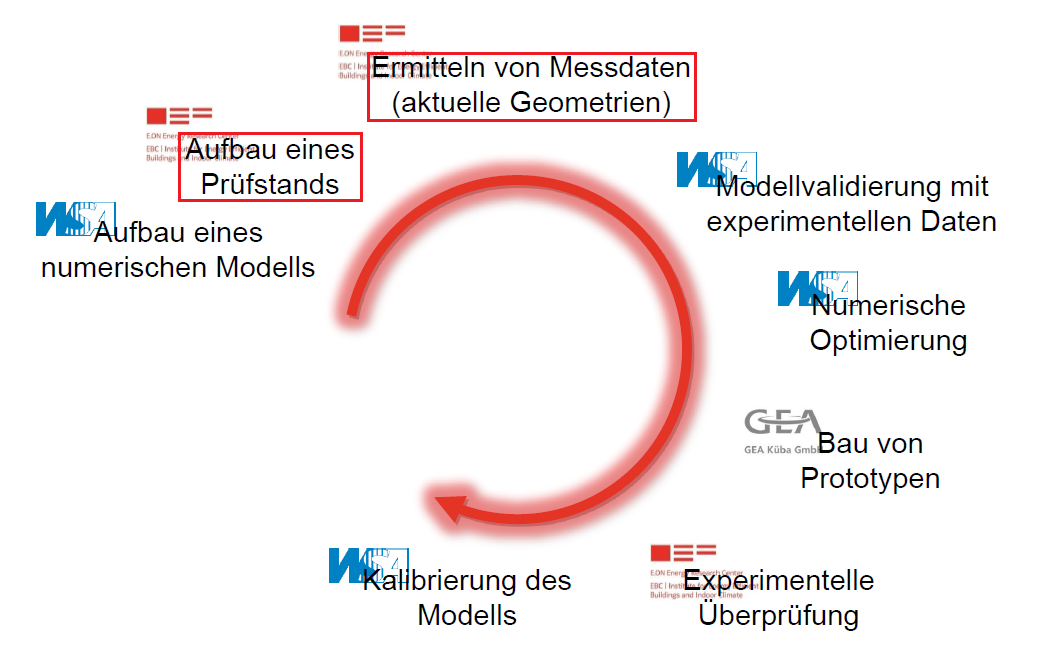
\includegraphics[width=0.80\textwidth]{Pictures/Projektablauf.png}
	\caption{Aufgabenpakete im Projektzyklus.\citep{Freitag2015} Rot umrahmte Arbeitspakte werden in dieser Masterarbeit behandelt und durchgeführt.}
	\label{fig:Aufgabenpakete}
\end{figure}

Die Ziele dieses Forschungsvorhabens sind sowohl experimentelle als auch numerische Erkenntnisgewinne im Hinblick auf Reifbildungsvorgänge als auch verschiedener Abtaumethoden bei Luftkühlern in einem Kältekreislauf. Diese Erkenntnisse sollen in eine spätere Datenbasis fließen, die zur energieeffizienten Auslegung von Luftkühlerkomponenten dienen wird.

Das WSA übernimmt hierbei die Entwicklung eines numerischen Simulationsmodelles. Das EBC ist verantwortlich für den Aufbau eines Abtauprüfstand zur Validierung der Simulationsergebnisse. Hierzu wurde bereits in einer vorhergegangenen Masterarbeit von \citeauthor{Helmlinger2015} eine Kälteanlage geplant und in Betrieb genommen. Der Luftkühler ist hierbei in einer Klimakammer platziert, in der unterschiedlichste Raumbedingungen eingestellt werden können. Die Luftkühler können getauscht werden, um verschiedene Wärmetauscher-Varianten testen zu können.

Diese Masterarbeit umfasst, wie in Abbildung \ref{fig:Aufgabenpakete} dargestellt, die Arbeitspakete 

\begin{itemize}
\item	Aufbau (bzw. Optimierung) eines Prüfstandes
\item	Ermitteln von Messdaten.
\end{itemize}

Das Arbeitspaket \textit{Aufbau (bzw. Optimierung) eines Prüfstandes} unterteilt sich in 

\begin{itemize}
\item Entwicklung und Bau eines Wägesystems zur Messung und Bestimmung des 2D-Schwerpunktes der Eismenge im Luftkühler
\item Entwicklung und Implemtierung einer Speicher-Programmierbaren-Steuerung
\end{itemize}



